\subsection{complexwf\_\-t Struct Reference}
\label{structcomplexwf__t}\index{complexwf\_\-t@{complexwf\_\-t}}
{\tt \#include $<$bpm\_\-wf.h$>$}

Collaboration diagram for complexwf\_\-t:\nopagebreak
\begin{figure}[H]
\begin{center}
\leavevmode
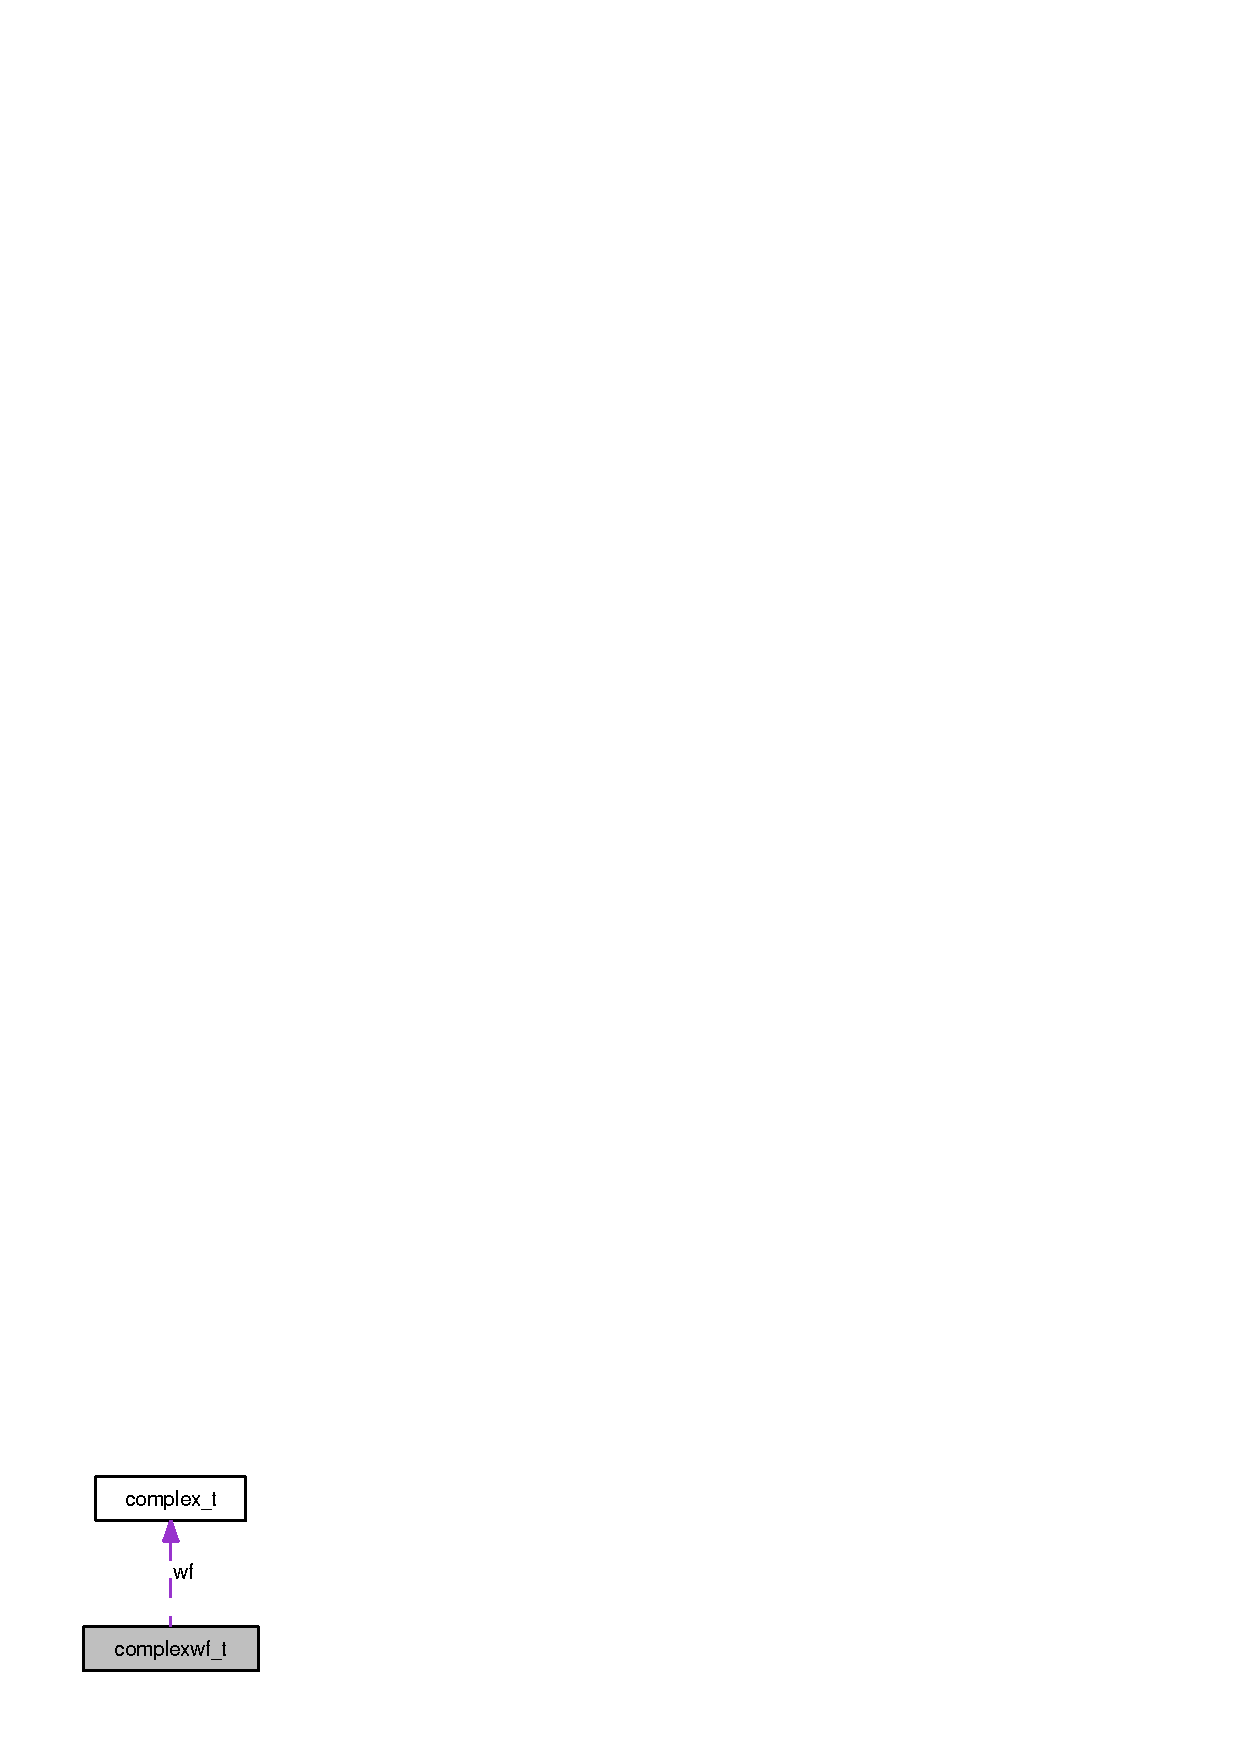
\includegraphics[width=64pt]{structcomplexwf__t__coll__graph}
\end{center}
\end{figure}


\subsubsection{Detailed Description}
Structure representing a waveform of complex numbers 

Definition at line 188 of file bpm\_\-wf.h.\subsubsection*{Data Fields}
\begin{CompactItemize}
\item 
int {\bf ns}
\item 
double {\bf fs}
\item 
{\bf complex\_\-t} $\ast$ {\bf wf}
\end{CompactItemize}


\subsubsection{Field Documentation}
\index{complexwf\_\-t@{complexwf\_\-t}!ns@{ns}}
\index{ns@{ns}!complexwf_t@{complexwf\_\-t}}
\paragraph[ns]{\setlength{\rightskip}{0pt plus 5cm}int {\bf complexwf\_\-t::ns}}\hfill\label{structcomplexwf__t_6ca8e343a776b345f6753539f2c2d865}


The number of samples in the waveform 

Definition at line 189 of file bpm\_\-wf.h.

Referenced by add\_\-mode\_\-response(), complexfft(), complexwf(), complexwf\_\-add(), complexwf\_\-add\_\-ampnoise(), complexwf\_\-add\_\-cwtone(), complexwf\_\-add\_\-dcywave(), complexwf\_\-add\_\-noise(), complexwf\_\-add\_\-phasenoise(), complexwf\_\-bias(), complexwf\_\-compat(), complexwf\_\-copy(), complexwf\_\-copy\_\-new(), complexwf\_\-divide(), complexwf\_\-getamp(), complexwf\_\-getamp\_\-new(), complexwf\_\-getimag(), complexwf\_\-getimag\_\-new(), complexwf\_\-getphase(), complexwf\_\-getphase\_\-new(), complexwf\_\-getreal(), complexwf\_\-getreal\_\-new(), complexwf\_\-multiply(), complexwf\_\-print(), complexwf\_\-reset(), complexwf\_\-scale(), complexwf\_\-setfunction(), complexwf\_\-setimag(), complexwf\_\-setreal(), complexwf\_\-setvalues(), complexwf\_\-subset(), complexwf\_\-subtract(), ddc(), fit\_\-fft(), fit\_\-fft\_\-prepare(), generate\_\-bpmsignal(), get\_\-mode\_\-response(), and realfft().\index{complexwf\_\-t@{complexwf\_\-t}!fs@{fs}}
\index{fs@{fs}!complexwf_t@{complexwf\_\-t}}
\paragraph[fs]{\setlength{\rightskip}{0pt plus 5cm}double {\bf complexwf\_\-t::fs}}\hfill\label{structcomplexwf__t_9b20d8d502ef45df29ecd14781cf06ac}


The sampling frequency 

Definition at line 190 of file bpm\_\-wf.h.

Referenced by complexwf(), complexwf\_\-add\_\-cwtone(), complexwf\_\-add\_\-dcywave(), complexwf\_\-compat(), complexwf\_\-copy\_\-new(), complexwf\_\-getamp\_\-new(), complexwf\_\-getimag\_\-new(), complexwf\_\-getphase\_\-new(), complexwf\_\-getreal\_\-new(), complexwf\_\-print(), complexwf\_\-setfunction(), complexwf\_\-subset(), ddc(), fit\_\-fft(), fit\_\-fft\_\-prepare(), generate\_\-bpmsignal(), and get\_\-mode\_\-response().\index{complexwf\_\-t@{complexwf\_\-t}!wf@{wf}}
\index{wf@{wf}!complexwf_t@{complexwf\_\-t}}
\paragraph[wf]{\setlength{\rightskip}{0pt plus 5cm}{\bf complex\_\-t}$\ast$ {\bf complexwf\_\-t::wf}}\hfill\label{structcomplexwf__t_9e02fc80ee52a0035e84bbc1a9fbb128}


Pointer to an array of integers which hold the samples 

Definition at line 191 of file bpm\_\-wf.h.

Referenced by add\_\-mode\_\-response(), complexfft(), complexwf(), complexwf\_\-add(), complexwf\_\-add\_\-ampnoise(), complexwf\_\-add\_\-cwtone(), complexwf\_\-add\_\-dcywave(), complexwf\_\-add\_\-noise(), complexwf\_\-add\_\-phasenoise(), complexwf\_\-bias(), complexwf\_\-copy(), complexwf\_\-copy\_\-new(), complexwf\_\-delete(), complexwf\_\-divide(), complexwf\_\-getamp(), complexwf\_\-getamp\_\-new(), complexwf\_\-getimag(), complexwf\_\-getimag\_\-new(), complexwf\_\-getphase(), complexwf\_\-getphase\_\-new(), complexwf\_\-getreal(), complexwf\_\-getreal\_\-new(), complexwf\_\-multiply(), complexwf\_\-print(), complexwf\_\-reset(), complexwf\_\-scale(), complexwf\_\-setfunction(), complexwf\_\-setimag(), complexwf\_\-setreal(), complexwf\_\-setvalues(), complexwf\_\-subset(), complexwf\_\-subtract(), downmix\_\-waveform(), fit\_\-fft(), fit\_\-fft\_\-prepare(), process\_\-caltone(), process\_\-waveform(), and realfft().

The documentation for this struct was generated from the following file:\begin{CompactItemize}
\item 
bpmwf/{\bf bpm\_\-wf.h}\end{CompactItemize}
